\chapter{Display}

In diesem Kapitel gehen wir auf das Display ein, das im \textbf{Spiegel AI} Projekt verwendet wird. Wir beschreiben die Spezifikationen, die Installation und die Anpassungen, die vorgenommen wurden.

\section{Spezifikationen}
Beschreiben Sie die technischen Spezifikationen des Displays.

\section{Installation}
Erläutern Sie den Prozess der Installation des Displays.

\section{Anpassungen}
Beschreiben Sie etwaige Anpassungen oder Modifikationen am Display.

\subsection{eventuell HTMl seite und Aufbau oder in Installation}
\subsection{Widget 1}
\subsection{Widget 2}
\subsection{Widget 3}
\subsection{Widget 4}
\subsection{Uhr Widget}
Erarbeitet von: Marcel Wagner \\ \\
\noindent
Die Implementierung des Uhrzeit Widgets für den Smart Mirror ist ein wichtiger Schritt zur Verbesserung der Funktionalität und Benutzerfreundlichkeit des Geräts. Ziel dieses Widgets ist es, die aktuelle Uhrzeit exakt und zuverlässig anzuzeigen. Wobei die Anzeige in Echtzeit aktualisiert werden muss, um stets die genaue Uhrzeit widerzuspiegeln.\\ \\
Die Implementierung dieses Widgets basierte auf der Nutzung von JavaScript zur Echtzeitaktualisierung der Uhrzeit und HTML zur Einbettung des Widgets in die Benutzeroberfläche des Smart Mirrors. Desweiteren wurde CSS benutzt um das Widget zu formatieren. Die JavaScript Funktion sorgt dafür, dass die Uhrzeit jede Sekunde aktualisiert wird, während das HTML Dokument die Struktur definiert. Abschließend definiert die CSS Datei das Styling des Widgets. \\ \\
\noindent
Während der Entwicklung des Widgets traten mehrere Herausforderungen auf. Eine der größten Herausforderungen bestand darin, sicherzustellen, dass die Uhrzeit in Echtzeit und ohne Verzögerung aktualisiert wird. Dies war besonders wichtig, um die Genauigkeit der angezeigten Zeit zu gewährleisten. Die Verwendung der 'setTimeout' Funktion in JavaScript ermöglicht eine wiederholte Ausführung der Aktualisierungsfunktion in einem festgelegten Intervall von einer Sekunde, wodurch eine kontinuierliche und genaue Aktualisierung der Uhrzeit sichergestellt wurde.
Eine weitere Herausforderung war die exakte Zeitanzeige, insbesondere hierbei ist wichtig die Erwähnung der Formatierung der Uhrzeit, um sicherzustellen, dass Stunden, Minuten und Sekunden stets zweistellig angezeigt werden. Durch die Verwendung der 'padStart' Methode konnten die Zahlen auf eine konstante Länge von zwei Stellen gebracht werden, indem bei Bedarf führende Nullen hinzugefügt werden. Dies gewährleistete eine konsistente und gut lesbare Anzeige.\\ \\
\noindent
Die Implementierung des Uhrzeit Widgets verlief erfolgreich und erfüllt die gestellten Anforderungen. Die Uhrzeit wird zuverlässig und exakt in Echtzeit angezeigt. Das Widget integriert sich nahtlos in die Benutzeroberfläche des Smart Mirrors und bietet eine klare und gut lesbare Darstellung der aktuellen Uhrzeit.
Insgesamt stellt das Uhrzeit Widget eine wesentliche Funktionalität des Smart Mirrors dar. Der nachfolgenden Abbildung 1 kann das Implementierte Uhrzeit Widget auf der HTML Seite entnommen werden.

\begin{figure}[h]
    \centering
    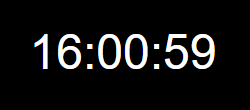
\includegraphics[width=0.4\textwidth]{pictures/time_widget.png}
  \captionsetup{justification=centering, labelformat=simple, singlelinecheck=false}
    \caption{ Uhrzeit Widget\\ Quelle: eigene Darstellung}
\end{figure}

\subsection{Verkehrsinformation}
Erarbeitet von: Marcel Wagner \\ \\
\noindent
Die Implementierung des Stau-Widgets auf dem Smart Mirror stellt einen wichtigen Schritt dar, um den Nutzern eine umfassende und zuverlässige Quelle für aktuelle Verkehrsinformationen zur Verfügung zu stellen. Das Widget wurde speziell entwickelt, um eine Echtzeitübersicht über die Verkehrslage in Regensburg zu bieten, was insbesondere für Pendler und Reisende von großem Nutzen ist. Durch die Verwendung von JavaScript wurde eine nahtlose Integration mit der OpenStreetMap Overpass API realisiert, die als zuverlässige Datenquelle für Verkehrsdaten dient. \\ \\
\noindent
Die Strategie hinter der Implementierung war zweigleisig: Zum einen wurde eine sofortige Aktualisierung der Verkehrsinformationen beim Laden der Seite implementiert, um den Nutzern bei jedem Besuch des Smart Mirrors die aktuellsten Daten bereitzustellen. Zum anderen erfolgt eine regelmäßige automatische Aktualisierung alle fünf Minuten, um sicherzustellen, dass die angezeigten Informationen kontinuierlich aktuell gehalten werden. Dieser Ansatz gewährleistet eine hohe Aktualität und Relevanz der bereitgestellten Verkehrsinformationen. \\ \\
\noindent
Während der Entwicklung wurden mehrere Herausforderungen gemeistert, darunter die robuste Fehlerbehandlung, um sicherzustellen, dass Netzwerkprobleme oder API Ausfälle die Funktionalität des Widgets nicht beeinträchtigen. Ein besonderes Augenmerk lag auf der Gewährleistung einer stabilen und zuverlässigen Datenaktualisierung, die für eine nahtlose Benutzererfahrung entscheidend ist. \\ \\
\noindent
Das Verkehrs Widget präsentiert die Verkehrslage in einer klaren und intuitiven Benutzeroberfläche. Es informiert die Nutzer klar verständlich darüber, ob derzeit ein Stau vorliegt oder nicht, und bietet gegebenenfalls zusätzliche Informationen über Verkehrshindernisse oder Verkehrswarnungen. Diese klare visuelle Darstellung hilft den Nutzern, schnell zu erfassen, wie die aktuelle Verkehrssituation ihre geplante Route beeinflussen ist. \\ \\
\noindent
Insgesamt trägt das Verkehrs Widget erheblich zur Funktionalität und Benutzerfreundlichkeit des Smart Mirrors bei. Es bietet eine unverzichtbare Informationsquelle für die tägliche Routenplanung und unterstützt die Nutzer dabei, ihre Fahrtzeiten effizient zu optimieren. Das Implementierte Verkehrsinformationen Widget kann der nachfolgenden Abbildung entnommen werden. Diese Abbildung zeigt den Fall, dass aktuell gerade kein Stau  in den Straßen von Regensburg sind.

\begin{figure}[h]
    \centering
    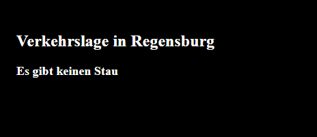
\includegraphics[width=0.4\textwidth]{pictures/traffic_widget.png}
  \captionsetup{justification=centering, labelformat=simple, singlelinecheck=false}
    \caption{Verkehrsinformations Widget\\ Quelle: eigene Darstellung}
\end{figure}

\subsection{Schlagzeilen}
\subsection{Tankstellen}


